\documentclass[12pt, a4paper]{article} %determina o tamanho da fonte, o tipo de papel e o tipo de documento.

\setlength{\parindent}{1.0 cm} %tamanho do espa\c{c}o para come\c{c}ar o parágrafo.
\setlength{\parskip}{0.5cm} %tamanho do espa\c{c}o entre os parágrafos.

%Aqui ficam os pacotes utilizados para formata\c{c}\~ao do documento de modo geral:

\usepackage[utf8]{inputenc} 
\usepackage{indentfirst} %Coloca espa\c{c}os nos inícios de parágrafos automaticamente. 
\usepackage[brazilian]{babel} %
\usepackage{amsmath}
\usepackage[hmargin=3cm, vmargin=2.5cm, bmargin=2.5cm]{geometry}
\usepackage{multicol}
\usepackage{graphicx} %para poder inserir imagens
\usepackage{subfig}
\usepackage{booktabs} 
\usepackage{hyperref} %para poder adicionar links e hiperlinks
\usepackage{float} %para poder posicionar as imagens
\usepackage{subfig} %para colocar duas imagens juntas

\usepackage{listings} %para poder incluir códigos
\usepackage{xcolor}
\definecolor{codegreen}{rgb}{0,0.6,0}
\definecolor{codegray}{rgb}{0.5,0.5,0.5}
\definecolor{codepurple}{rgb}{0.58,0,0.82}
\definecolor{backcolour}{rgb}{0.95,0.95,0.92}
\lstdefinestyle{mystyle}{
    backgroundcolor=\color{backcolour},   
    commentstyle=\color{codegreen},
    keywordstyle=\color{magenta},
    numberstyle=\tiny\color{codegray},
    stringstyle=\color{codepurple},
    basicstyle=\ttfamily\footnotesize,
    breakatwhitespace=false,         
    breaklines=true,                 
    captionpos=b,                    
    keepspaces=true,                 
    numbers=left,                    
    numbersep=5pt,                  
    showspaces=false,                
    showstringspaces=false,
    showtabs=false,                  
    tabsize=2,
    morecomment={l}[!],
    language=[77]Fortran,
}
\lstset{style=mystyle}

\begin{document} %come\c{c}a alguma coisa,neste caso, o documento, sempre importante lembrar de colocar o \end{} para n\~ao dar erro 
	
	\begin{titlepage}
		\begin{center}
\Huge{Universidade de S\~ao Paulo}\\
\large{Instituto de Física de S\~ao Carlos}\\
\vspace{20pt}
\vspace{200pt}
\textbf{Lista 5}\\
\vspace{8cm}
		\end{center}

\begin{flushleft}
\begin{tabbing}
Pedro Calligaris Delbem 5255417\\
\end{tabbing}
\vspace{0.5cm}
Professor: Attilio Cucchieri\\		
		\end{flushleft}
	
		\begin{center}
			\vspace{\fill}
	Junho de 2025	
		\end{center}
	\end{titlepage}

%####################################################################### SUMÁRIO
	\tableofcontents 
	\thispagestyle{empty}
	\newpage
%#########################################################################

    \section{Exerc\'icio 1}

        Tarefa: Na lista 5, foi considerado o po\c{c}o de potencial infinito no intervalo $[0, L]$, para uma part\'icula de massa $m$, ou seja, a equac\c{c}\~ao
        \begin{equation}
            -\frac{\hbar^{2}}{2m}\nabla^{2}\psi_{j}(x)=E_{j}\psi_{j}(x).
        \end{equation}
        Para encontrar as autofun\c{c}\~oes
        \begin{equation*}
            \psi_{j}(x) \propto \sin\left(\frac{j\pi x}{L}\right)
        \end{equation*}
         foi considerada a matriz
        \[
        \begin{pmatrix}
            -2 & 1 & 0 & \cdots & 0 \\
            1 & -2 & 1 & \cdots & 0 \\
            0 & 1 & -2 & \cdots & 0 \\
            \vdots & \vdots & \ddots & \ddots & \vdots \\
            0 & 0 & 0 & 1 & -2
        \end{pmatrix}
        \]
        Agora, considere a matriz
        \begin{equation}
        \begin{pmatrix}
            -1 & 1 & 0 & \cdots & 0 \\
            1 & -2 & 1 & \cdots & 0 \\
            0 & 1 & -2 & \cdots & 0 \\
            \vdots & \vdots & \ddots & \ddots & \vdots \\
            0 & 0 & 0 & 1 & -2
        \end{pmatrix}
        \end{equation}
        Que tipo de soluc\c{c}\~oes para o po\c{c}o de potencial infinito voc\^e espera encontrar nesse caso? Motive sua resposta.
        
        \textbf{Resposta:}

        Para um ponto no extremo inicial da grade, a discretiza\c{c}\~ao de diferen\c{c}as finitas para a primeira derivada \'e:
        \begin{equation}
            \frac{d\psi}{dx} \bigg|_{x=0} \approx \frac{\psi_1 - \psi_0}{h}
        \end{equation}
        A Condi\c{c}\~ao de Contorno de Neumann é:
        \begin{equation}
            \frac{d\psi}{dx} \bigg|_{x=0} = 0
        \end{equation}
        O que nos leva a
        \begin{equation}
            \psi_0 = \psi_1
        \end{equation}
        Substituindo isto na discretiza\c{c}\~ao de diferen\c{c}as finitas para a segunda derivada - no ponto $x_i$, temos:
        \begin{equation}
            \frac{d^2\psi}{dx^2} \bigg|_{x=x_1} \approx \frac{\psi_2 - 2\psi_1 + (\psi_1)}{h^2} = \frac{\psi_2 - \psi_1}{h^2}
        \end{equation}
        Que resulta em dois termos, justamente com os coeficientes -1 e 1, que temos na matriz dada.
        Logo, espera-se que a solu\c{c}\~ao seja tal que obede\c{c}a a condi\c{c}\~ao de contorno de Neumann e portanto o resultado ser\'a:
        \begin{equation*}
            \psi_{j}(x) \propto \cos\left(\frac{j\pi x}{2L}\right)
        \end{equation*}

    \section{Exercício 2}

        Tarefa: Usando o \textit{power method} e a matriz (2), calcule a energia do estado fundamental $E_{0}$ com precis\~ao de $10^{-4}$. Compare o resultado com o valor exato. Fa\c{c}a um gr\'afico da autofunc\c{c}\~ao normalizada e compare com a soluc\c{c}\~ao exata.

        O c\'odigo foi compilado com o comando:

    gfortran -ffree-form -ffree-line-length-none P2-5255417-ex-2.f90 -Wall -Wextra -pedantic -o P2-5255417-ex-2.exe

        Resultados:

        Utilizou-se N=100000 como se fosse N=infinito, obtendo a energia:
        \begin{figure}[H]
            \centering
            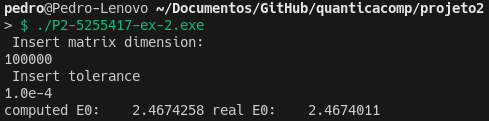
\includegraphics[width=0.8\textwidth]{../images/ex2.png}
        \end{figure}
        E obteve-se a seguinte autofun\c{c}\~ao:
        \begin{figure}[H]
            \centering
            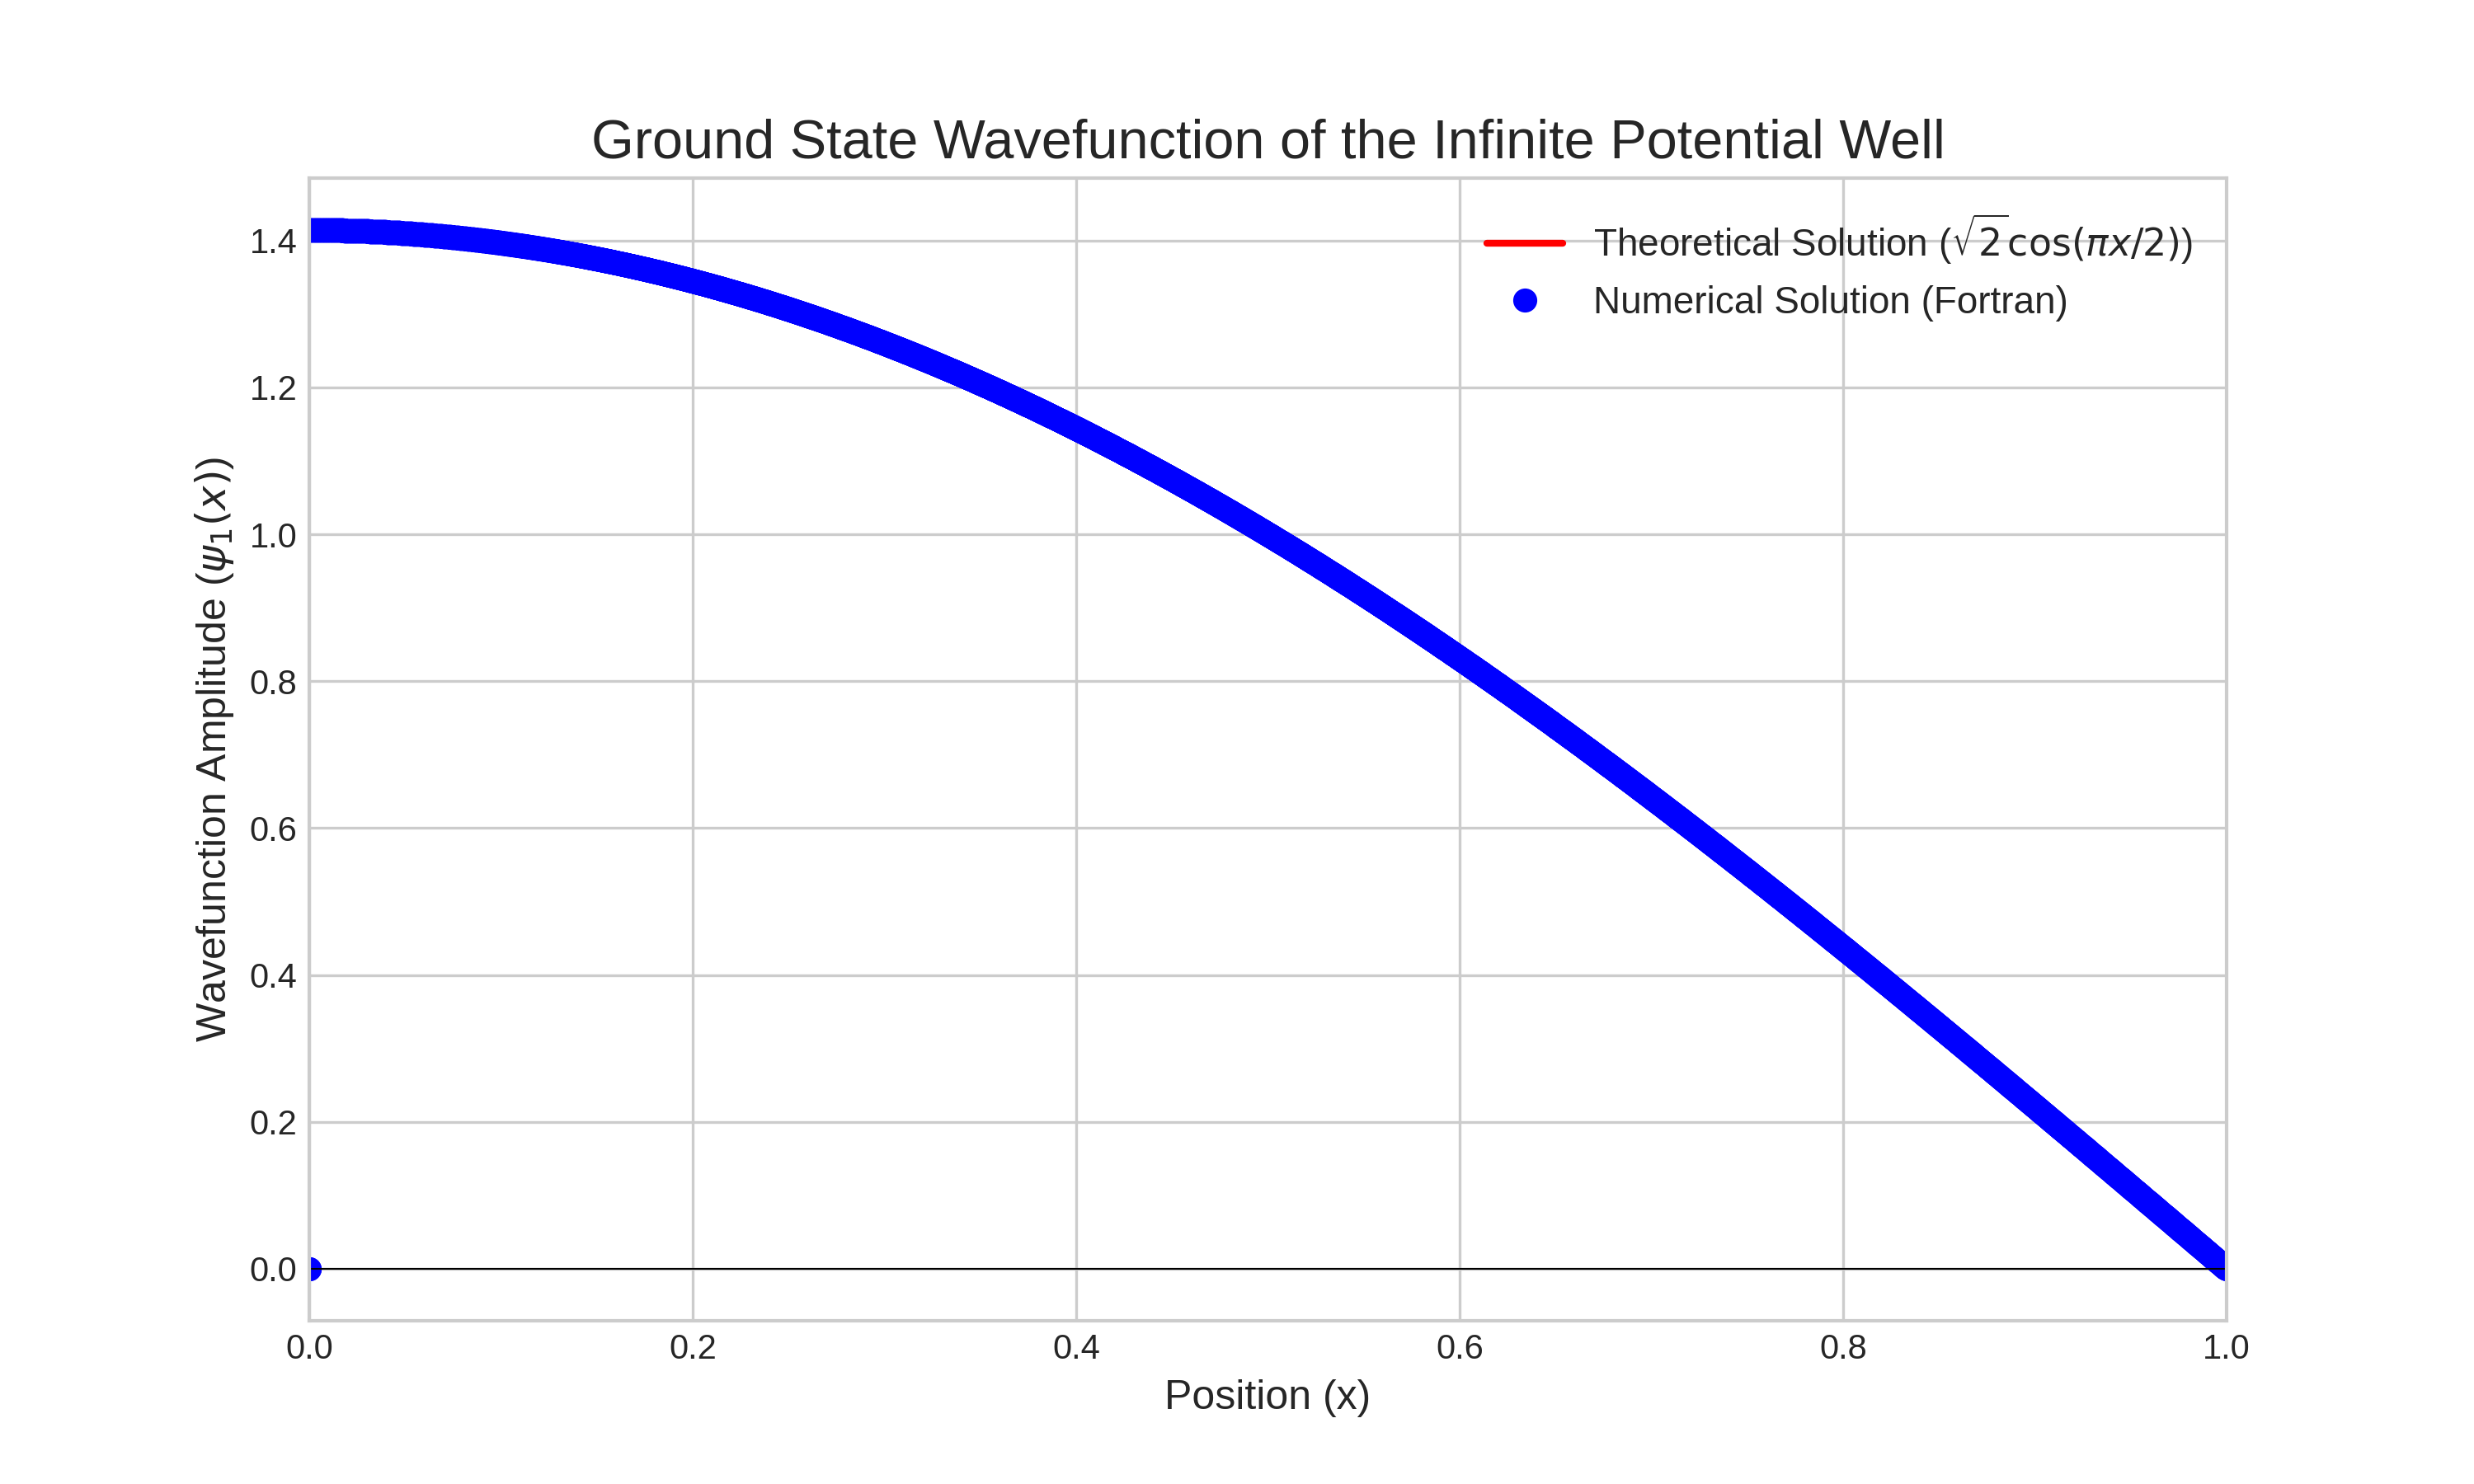
\includegraphics[width=0.8\textwidth]{../images/wavefunction_plot.png}
        \end{figure}

        V\^e-se que a fun\c{c}\~ao anal\'itica e a num\'erica se sobrep\~oe totalmente, de modo que o m\'etodo num\'erico corresponde perfeitamente à fun\c{c}\~ao anal\'itica conhecida. (O autovetor resultante foi salvo no arquivo "P2-5255417-ex-2-results.txt")

    \section{Exerc\'icio 3}

        Tarefa: Considere o m\'etodo de Householder, estudado na lista 6. Naquele caso, para os elementos fora da diagonal $k_{i}$, foi usado o sinal oposto de $a_{i-1,i}$. O que acontece quando o sinal de $k_{i}$ \'e o mesmo de $a_{i-1,i}$? Estude o problema para a mesma matriz considerada na lista 6, ou seja
        \[
        A =
        \begin{pmatrix}
        -\frac{5}{2} & \frac{4}{3} & -\frac{1}{12} & 0 & 0 & 0 \\
        \frac{4}{3} & -\frac{5}{2} & \frac{4}{3} & -\frac{1}{12} & 0 & 0 \\
        -\frac{1}{12} & \frac{4}{3} & -\frac{5}{2} & \frac{4}{3} & -\frac{1}{12} & 0 \\
        0 & -\frac{1}{12} & \frac{4}{3} & -\frac{5}{2} & \frac{4}{3} & -\frac{1}{12} \\
        0 & 0 & -\frac{1}{12} & \frac{4}{3} & -\frac{5}{2} & \frac{4}{3} \\
        0 & 0 & 0 & -\frac{1}{12} & \frac{4}{3} & -\frac{5}{2}
        \end{pmatrix}
        \]
        Qual \'e a relac\c{c}\~ao entre a matriz tridiagonal obtida neste caso e a matriz tridiagonal obtida na lista 6?
        

        Resultados:

        Obteve-se os seguintes resultados:
        \begin{figure}[H]
            \centering
            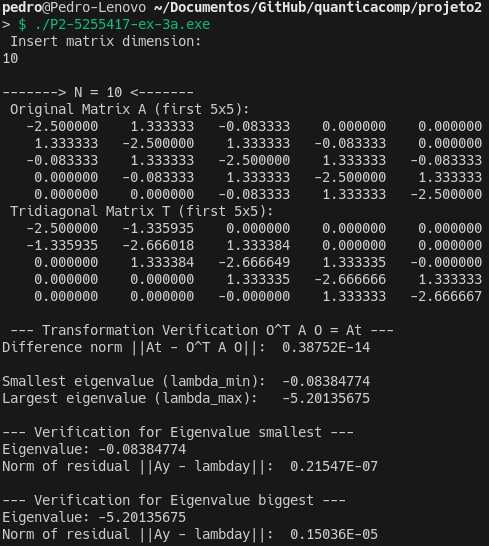
\includegraphics[width=0.8\textwidth]{../images/ex3a-10.png}
        \end{figure}
        \begin{figure}[H]
            \centering
            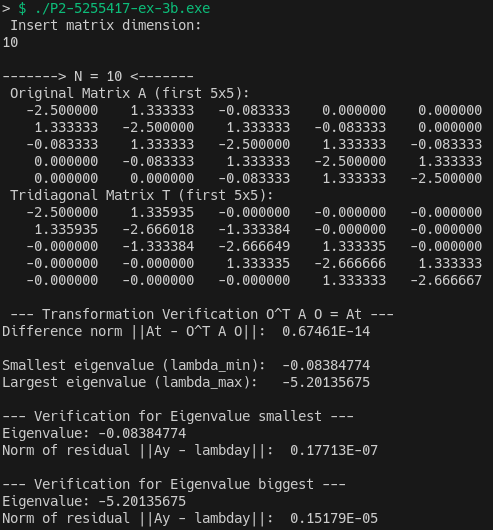
\includegraphics[width=0.8\textwidth]{../images/ex3b-10.png}
        \end{figure}
        \begin{figure}[H]
            \centering
            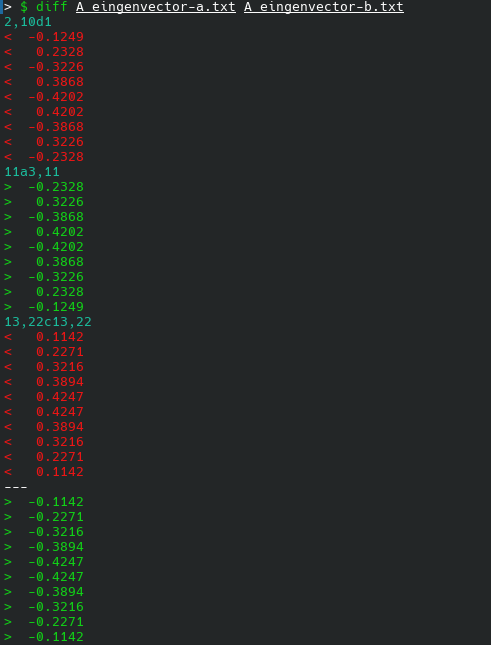
\includegraphics[width=0.8\textwidth]{../images/diffA10.png}
        \end{figure}
        \begin{figure}[H]
            \centering
            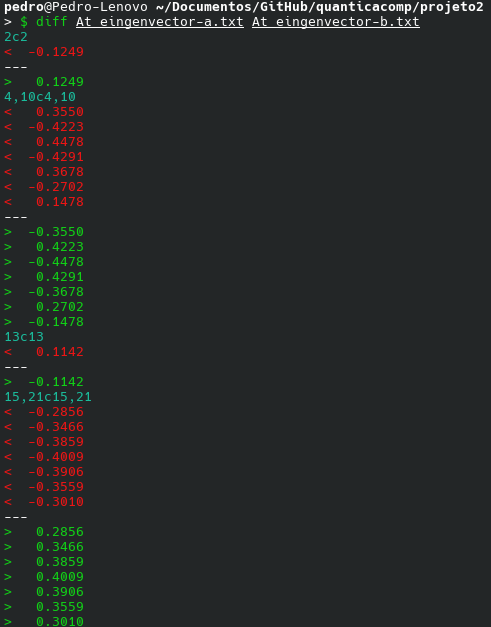
\includegraphics[width=0.8\textwidth]{../images/diffAt10.png}
        \end{figure}

        Nota-se que todas as verifica\c{c}\~oes - em ambos os c\'odigos - resultaram em valores pequenos, mostrando que o m\'etodo funcionou bem para ambos os c\'odigos.
        Entretando, ao comparar os arquivos que cont\^em os autovetores resultantes ("At\_eingenvectors-a.txt" e "A\_eingenvectors-a.txt" para o sinal original e "At\_eingenvectors-b.txt" e "A\_eingenvectors-b.txt" para o sinal modificado) - al\'em de comparar as matrizes impressas como resultado dos c\'odigos -  percebe-se que há uma diferen\c{c}a de sinal em alguns elementos da matriz, enquanto os autovetores apresentam - al\'em da diferen\c{c}a de sinal - uma invers\~ao da "ordem" dos elementos (apesar de serem os mesmos).
        Deste modo, percebe-se que o m\'etodo funcionou bem para ambos os sinais - encontrando, para cada sinal, uma das duas solu\c{c}\~oes poss\'iveis. O erro esperado - devido ao erro de subtra\c{c}\~ao num\'erica - n\~ao foi um problema devido a utiliza\c{c}\~ao de dupla preciss\~ao nas contas.



\end{document}